\chapter*{Acknowledgements}
\addcontentsline{toc}{chapter}{Acknowledgements}

\section*{Institutions}

We thank Columbia University along with the Departments of
Statistics and Political Science, the Applied Statistics Center, the
Institute for Social and Economic Research and Policy ({\sc iserp}),
and the Core Research Computing Facility.

\section*{Grants}

\Stan was supported in part by 
%
the U.~S.\ Department of Energy 
({\small DE-SC0002099}), 
%
the U.~S.\ National Science Foundation 
{\small ATM-0934516}
``Reconstructing Climate from Tree Ring Data.''
and 
%
the U.~S.\ Department of Education Institute of Education Sciences 
({\small ED-GRANTS-032309-005}:
 ``Practical Tools for Multilevel Hierarchical Modeling in Education
 Research'' and
 {\small R305D090006-09A}:
 ``Practical solutions for missing data'').
%
The high-performance computing
facility on which we ran evaluations was made possible through 
a grant from the U.~S.\ National Institutes of Health 
({\small 1G20RR030893-01}:
 ``Research Facility Improvement Grant'').

\Stan is currently supported in part by a grant from the National
Science Foundation (CNS-1205516)

\section*{Individuals}

We thank John Salvatier for pointing us to automatic differentiation
and \HMC in the first place.  And a special thanks to Kristen van
Leuven (formerly of Columbia's ISERP) for help preparing our initial
grant proposals.

\subsection*{Code  and Doc Patches}

Thanks for bug reports, code patches, pull requests, and diagnostics
to: 
Ethan Adams, 
Avraham Adler,
Jeffrey Arnold, 
Jarret Barber, 
David R.~Blair, 
Ross Boylan, 
Eric N.~Brown, 
Devin Caughey, 
Ctross (GitHub ID), 
Robert J.\ Goedman, 
Marco Inacio, 
B.~Harris, 
Kevin Van Horn, 
Andrew Hunter, 
Filip Krynicki
Dan Lakeland, 
Devin Leopold, 
Nathanael I.~Lichti,
Titus van der Malsburg,
P.~D.~Metcalfe, 
Linas Mockus,
Jeffrey Oldham, 
Fernando H.~Toledo, 
and Zhenming Su.

Thanks for documentation bug reports and patches to: 
Jeffrey Arnold,
Asim, 
Jarret Barber, 
Guido Biele,
Luca Billi, 
Eric C.~Brown, 
David Chudzicki,
Andria Dawson, 
Seth Flaxman, 
Wayne Folta, 
Mauricio Garnier-Villarreal,
Herra Huu,
Marco Inacio, 
Louis Luangkesorn, 
Mitzi Morris,
Tamas Papp, 
Sergio Polini,
Sean O'Riordain, 
Cody Ross, 
Mike Ross, 
Nathan Sanders, 
Terrance Savitsky,
Janne Sinkkonen, 
Dan Stowell, 
Dougal Sutherland, 
Andrew J.~Tanentzap,
Shravan Vashisth, 
Matt Wand,
Sebastian Weber, and
Howard Zail.

Thanks to Kevin van Horn for install instructions for Cygwin and to
Kyle Foreman for instructions on using the MKL compiler.


\subsection*{Bug Reports}

We're really thankful to everyone who's had the patience to try
to get Stan working and reported bugs.  All the gory details are
available from Stan's issue tracker at the following URL.
%
\begin{quote}
\url{https://github.com/stan-dev/stan/issues}
\end{quote}




\vfill
\begin{center}
\hfill
\begin{minipage}[b]{2in}
  \footnotesize {\it Stanislaw Ulam, namesake of \Stan and co-inventor
    of Monte Carlo methods \citep{MetropolisUlam:1949}, shown here
    holding the Fermiac, Enrico Fermi's physical Monte Carlo simulator
    for neutron diffusion.}
  \\[3pt] \mbox{ } \hfill
  {\scriptsize Image from \citep{Giesler:2000}.}
\end{minipage} \ \ \ \ \ 
\begin{minipage}[b]{1.5in} \mbox{ } \hfill
  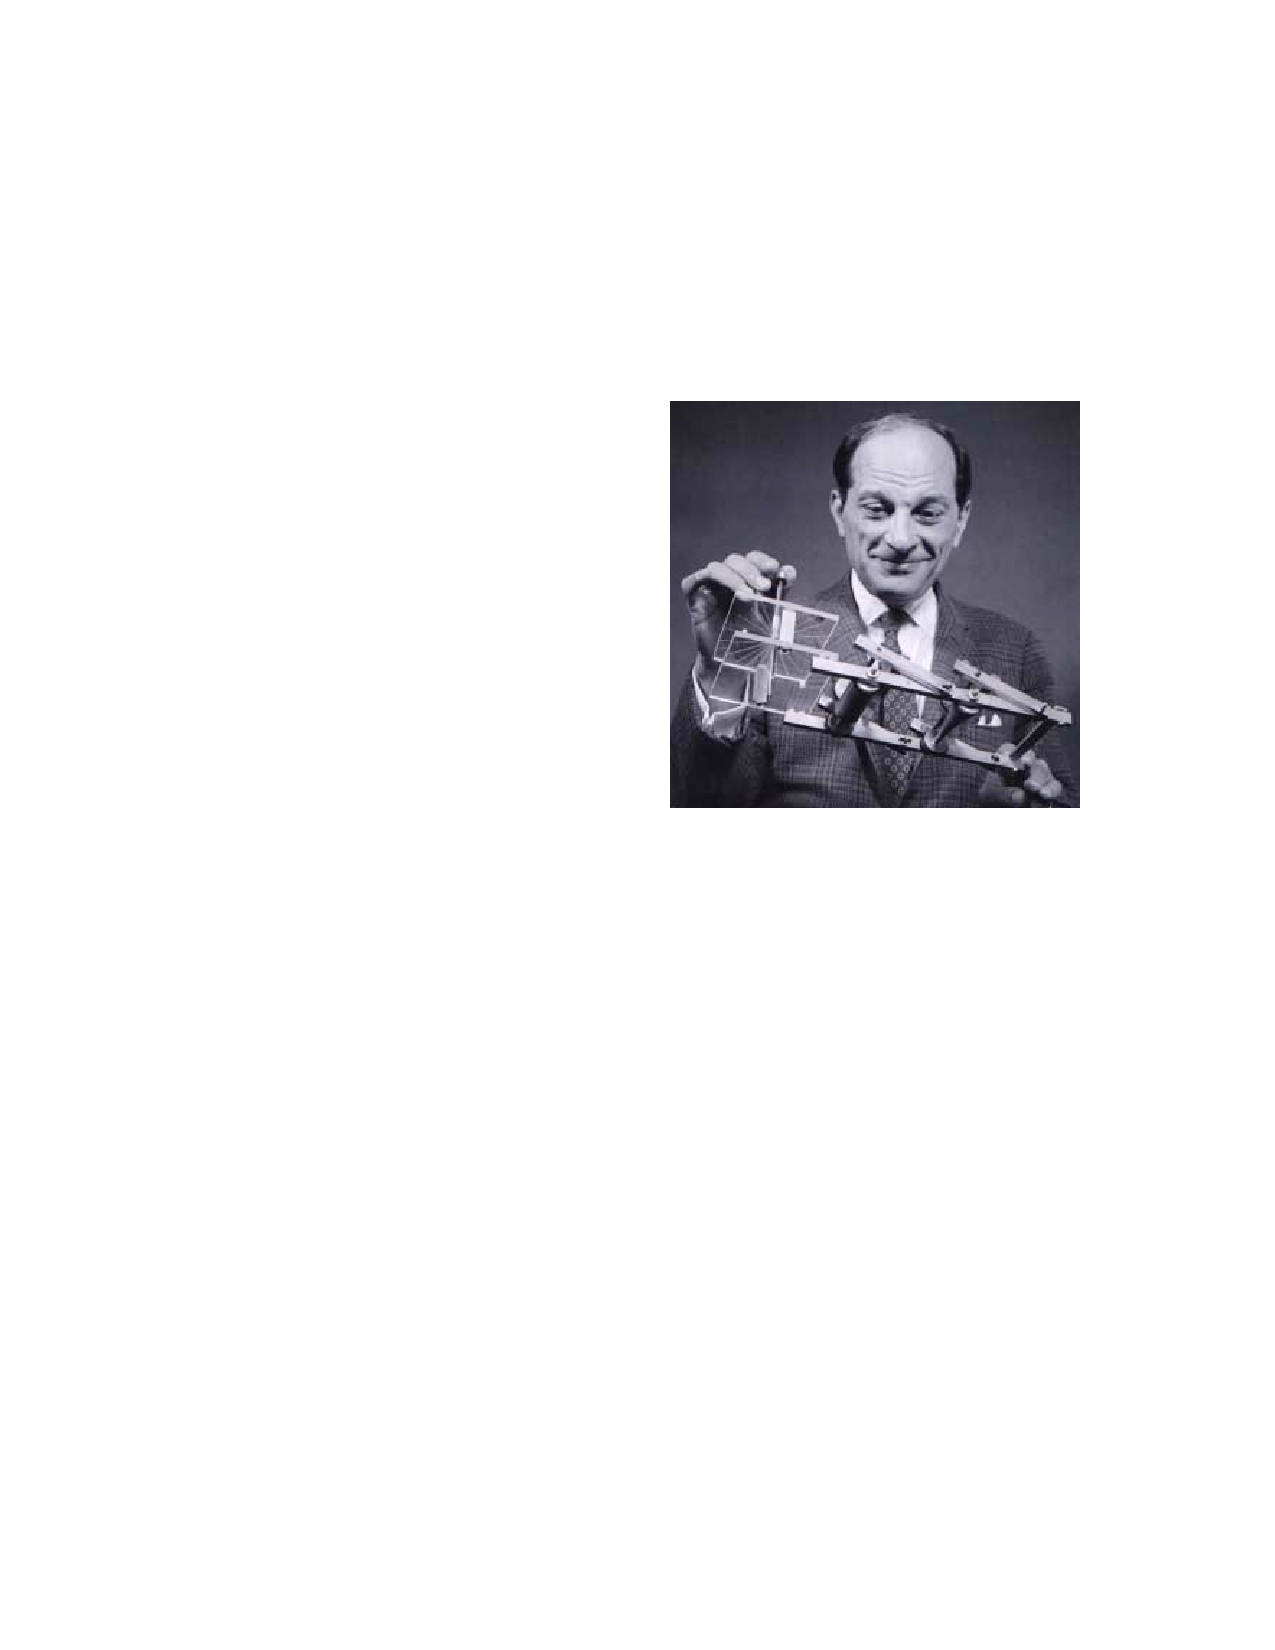
\includegraphics[width=1.5in]{../../../logos/ulam-fermiac.pdf}
\end{minipage} 
\end{center}
